\documentclass[a4paper]{article}
\usepackage[english]{babel}
\usepackage[utf8]{inputenc}

% mathermatics
\usepackage{amssymb} % useful math symbols
\usepackage{amsmath} % more useful math

% references and equation numbering
\usepackage{hyperref}
\usepackage{cleveref}
\usepackage{autonum}

% graphics
\usepackage{graphicx}
\usepackage{float}    % for more accurate graphics placement
\usepackage{fancyhdr} % for top header

% formatting
\usepackage{enumitem} % provides easy change of labels in enumerate environment
\usepackage[top=3cm, bottom=4cm, width=17cm]{geometry} % for smaller page margins

% colors
\usepackage{xcolor}

%% coding
% 
% see https://github.com/gpoore/minted for info
% uncomment this after you have completed the required installation
%
\usepackage{minted} 
\definecolor{codeBgColor}{RGB}{240,240,240}
%



% very simple alias, \ex{} becomes the same as \subsubsection*{}
% TIP: remove the * in the line below if you want it numbered
\newcommand{\ex}[1]{\subsubsection*{#1}}




%Begining of the document
\begin{document}

\pagestyle{fancy} % use pagestyle with simple header (from fancyhdr)

%\pagenumbering{gobble} % uncomment to remove pagenumbering (in case of single page document)
\fancyhead[L]{TMA4140 Diskret Matematikk}
\fancyhead[C]{\textbf{Øving 3}}
\fancyhead[R]{Otto Lote 748704}


\subsection*{Section 3.1}
\ex{Exercise 53}

\begin{enumerate}[label=\alph*)]
    \item Total: 2 quarters, 1 penny (51c)

    \item Total: 2 quarters, 1 dimes, 1 nickel, 4 pennies (69c)

    \item Total: 3 quarters, 1 penny (76c)

    \item Total: 2 quarters, 1 dime (60c)
\end{enumerate}


\ex{Exercise 55}

\begin{enumerate}[label=\alph*)]
    \item Total: 2 quarters, 1 penny (51c)

    \item Total: 2 quarters, 1 dime, 9 pennies (69c)

    \item Total: 3 quarters, 1 penny (76c)

    \item Total: 2 quarters, 1 dime (60c)

        The fewest coins are given when \((n \, \mathrm{mod}25) \, \mathrm{mod} 10 \geq 5\)

\end{enumerate}


\ex{Exercise 56}

Proof by counterexample:

15c using the greedy algorithm would draw one 12c coin and 3 pennies, which is four coins, when one dime and one nickel would suffice. 


\vspace{1em}
\subsection*{Section 3.2}
\ex{Exercise 27}

\begin{enumerate}[label=\alph*)] % a b
    \item \(n \log(n^2 + 1) = \mathcal{O}(n\,2\log n) = \mathcal{O}(n\log n)\) \\
        \(\mathcal{O}(n^2 \log n + n \log n) = \mathcal{O}(n^2\log n)\)

    \item \((n\log n + 1)^2 = \mathcal{O}(n^2(\log n)^2) \)
        \((\log n + 1)(n^2 + 1) = \mathcal{O}(n^2 \log n) \)
        \( \mathcal{O}(n^2 \log n) + \mathcal{O}(n^2 (\log n)^2) =
            \mathcal{O}(n^2 (\log n)^2) \)
\end{enumerate}


\ex{Exercise 30} % c e

\begin{enumerate}[start=3, label=\alph*)] % start at c)
    \item \(|\lfloor x + 1/2 \rfloor | \leq C|x| \forall x > k\) is true for
            (among others) \(C = 2\) and \(k = 2\) \\
        \(C|\lfloor x + 1/2 \rfloor | \geq |x| \forall x > k\) is true for
            (among others) \(C = 2\) and \(k = 2\) \\ 
        Therefore both expressions is \(\Theta(x)\)

    \addtocounter{enumi}{1} % skip d)
    \item \( \log_2(x) = \frac{\log_{10}(x)}{\log_{10}(2)} \implies 
        C\log_{10}(x) \propto \log_2(x)\) which means they are both
        \(\Theta(\log x)\)
\end{enumerate}


\ex{Exercise 34}

\begin{enumerate}[label=\alph*)]
    \item 
        \begin{align}
            f(x) &= 3x^2 + x + 1 \\
            g(x) &= 3x^2 \\
            C_1|3x^2| &\leq |3x^2 + x + 1| \leq C_2|3x^2|, \forall x > k \\
            \intertext{Since \(k\) can be chosen freely we choose \(k > 0\) to get rid
                of absolute values}
            3C_1x^2 &\leq 3x^2 + x + 1 \leq 3C_2x^2, \forall x > k \\
            \intertext{We simplify and get}
            3C_1 &\leq 3 + \frac{1}{x} + \frac{1}{x^2} \leq 3C_2, \forall x > k \\
            \intertext{The constants \(C_1 = \frac{1}{2}, C_2 = 2, k = 1\) is a solution}
        \end{align}

    \item {
        \texttt{loglog} in matlab is a nice way to plot this
        \begin{minted}{matlab}
x = logspace(-1,2);
g = 3*x.^2;
f1 = 1.5*x.^2 + 0.5*x + 0.5;
f2 = 6*x.^2 + 2*x + 2;
loglog(x,f1, x, g, x, f2);
legend('C_1 f(x)','g(x)','C_2 f(x)');
        \end{minted}
        \begin{figure}[H]
            \centering
            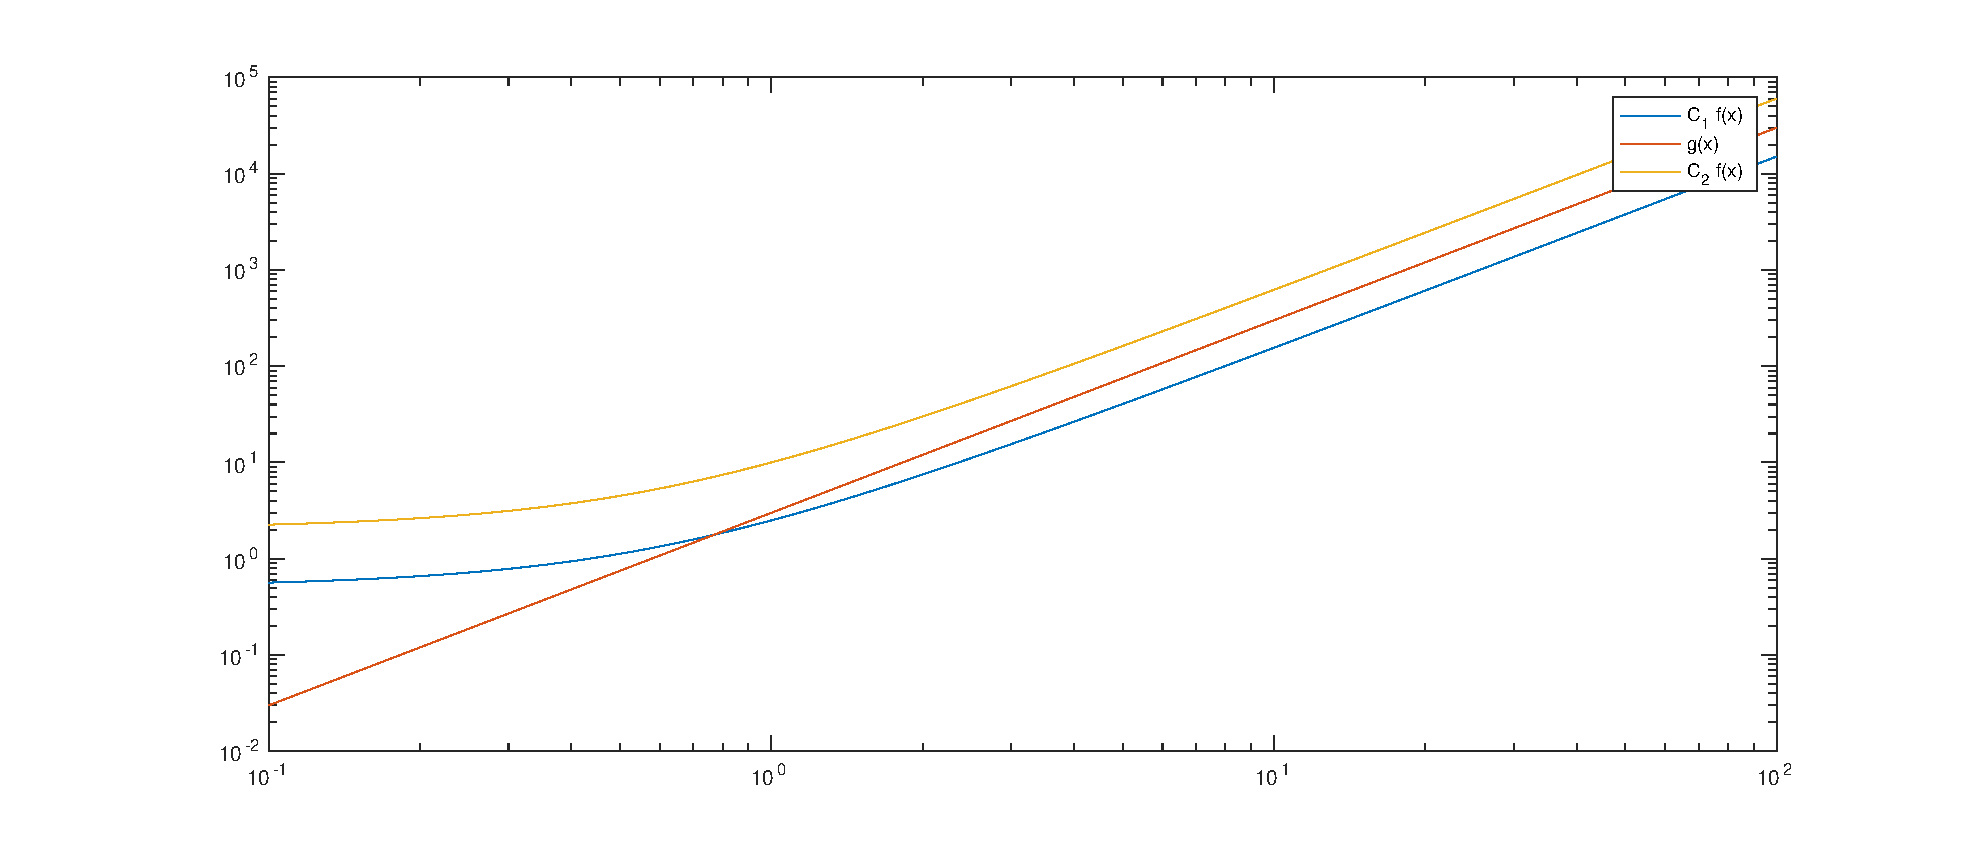
\includegraphics[width=0.7\textwidth]{ex34b.eps}
            \caption{\(f(x) = \Theta(3x^2)\) as we see here for \(x > 10^0 = 1\)}
        \end{figure}
    }
\end{enumerate}


\ex{Exercise 42}

\begin{align}
    \intertext{From \(f(x) = \mathcal{O}(g(x))\) we have that}
    \exists C, k \quad \text{such\ that} \quad C|g(x)| &\geq |f(x)|, \quad \forall x > k \\
    \intertext{If \(2^{f(x)} = \mathcal{O}(2^{g(x)})\) then the following must be true}
    C|2^{g(x)}| &\geq |2^{f(x)}| \\
    \intertext{\(2^a > 0, \,  \forall a\) so we can ignore absolute values}
    \log_2 C + \log_22^{g(x)} &\geq \log_22^{f(x)} \\
    \log_2 C + g(x) &\geq f(x) \\
    \intertext{For large values of \(x\), \(\log_2 C\) becomes insignificant,
        which means that \(g(x) \geq f(x)\) must hold for large \(x\) if \(2^{f(x)}
        = \mathcal{O}(2^{g(x)})\)}
    \intertext{Since \(f(x) = \mathcal{O}(g(x))\) does not imply \(g(x) \geq
        f(x), \, \forall x > k\) then it does not follow from \(f(x) =
        \mathcal{O}(g(x))\) that \(2^{f(x)} = \mathcal{O}(2^{g(x)})\)}
\end{align}


\subsection*{Section 4.1}
\ex{Exercise 11}

\begin{enumerate}[label=\alph*)]
    \item \(11 + 80 \mod 12 = 7\) \\
        The clock reads 7:00

    \item \(12 + 40 \mod 12 = 4\) \\
        The clock reads 4:00

    \item \(6 + 100 \mod 12 = 10\) \\
        The clock reads 10:00
\end{enumerate}



%% uncomment this if you need references. Edit the .bbl file with your references
%% and use "\cite{bibitem-label}" to cite
%\bibliography{template}

\end{document}

